\documentclass[1p]{elsarticle_modified}
%\bibliographystyle{elsarticle-num}

%\usepackage[colorlinks]{hyperref}
%\usepackage{abbrmath_seonhwa} %\Abb, \Ascr, \Acal ,\Abf, \Afrak
\usepackage{amsfonts}
\usepackage{amssymb}
\usepackage{amsmath}
\usepackage{amsthm}
\usepackage{scalefnt}
\usepackage{amsbsy}
\usepackage{kotex}
\usepackage{caption}
\usepackage{subfig}
\usepackage{color}
\usepackage{graphicx}
\usepackage{xcolor} %% white, black, red, green, blue, cyan, magenta, yellow
\usepackage{float}
\usepackage{setspace}
\usepackage{hyperref}

\usepackage{tikz}
\usetikzlibrary{arrows}

\usepackage{multirow}
\usepackage{array} % fixed length table
\usepackage{hhline}

%%%%%%%%%%%%%%%%%%%%%
\makeatletter
\renewcommand*\env@matrix[1][\arraystretch]{%
	\edef\arraystretch{#1}%
	\hskip -\arraycolsep
	\let\@ifnextchar\new@ifnextchar
	\array{*\c@MaxMatrixCols c}}
\makeatother %https://tex.stackexchange.com/questions/14071/how-can-i-increase-the-line-spacing-in-a-matrix
%%%%%%%%%%%%%%%

\usepackage[normalem]{ulem}

\newcommand{\msout}[1]{\ifmmode\text{\sout{\ensuremath{#1}}}\else\sout{#1}\fi}
%SOURCE: \msout is \stkout macro in https://tex.stackexchange.com/questions/20609/strikeout-in-math-mode

\newcommand{\cancel}[1]{
	\ifmmode
	{\color{red}\msout{#1}}
	\else
	{\color{red}\sout{#1}}
	\fi
}

\newcommand{\add}[1]{
	{\color{blue}\uwave{#1}}
}

\newcommand{\replace}[2]{
	\ifmmode
	{\color{red}\msout{#1}}{\color{blue}\uwave{#2}}
	\else
	{\color{red}\sout{#1}}{\color{blue}\uwave{#2}}
	\fi
}

\newcommand{\Sol}{\mathcal{S}} %segment
\newcommand{\D}{D} %diagram
\newcommand{\A}{\mathcal{A}} %arc


%%%%%%%%%%%%%%%%%%%%%%%%%%%%%5 test

\def\sl{\operatorname{\textup{SL}}(2,\Cbb)}
\def\psl{\operatorname{\textup{PSL}}(2,\Cbb)}
\def\quan{\mkern 1mu \triangleright \mkern 1mu}

\theoremstyle{definition}
\newtheorem{thm}{Theorem}[section]
\newtheorem{prop}[thm]{Proposition}
\newtheorem{lem}[thm]{Lemma}
\newtheorem{ques}[thm]{Question}
\newtheorem{cor}[thm]{Corollary}
\newtheorem{defn}[thm]{Definition}
\newtheorem{exam}[thm]{Example}
\newtheorem{rmk}[thm]{Remark}
\newtheorem{alg}[thm]{Algorithm}

\newcommand{\I}{\sqrt{-1}}
\begin{document}

%\begin{frontmatter}
%
%\title{Boundary parabolic representations of knots up to 8 crossings}
%
%%% Group authors per affiliation:
%\author{Yunhi Cho} 
%\address{Department of Mathematics, University of Seoul, Seoul, Korea}
%\ead{yhcho@uos.ac.kr}
%
%
%\author{Seonhwa Kim} %\fnref{s_kim}}
%\address{Center for Geometry and Physics, Institute for Basic Science, Pohang, 37673, Korea}
%\ead{ryeona17@ibs.re.kr}
%
%\author{Hyuk Kim}
%\address{Department of Mathematical Sciences, Seoul National University, Seoul 08826, Korea}
%\ead{hyukkim@snu.ac.kr}
%
%\author{Seokbeom Yoon}
%\address{Department of Mathematical Sciences, Seoul National University, Seoul, 08826,  Korea}
%\ead{sbyoon15@snu.ac.kr}
%
%\begin{abstract}
%We find all boundary parabolic representation of knots up to 8 crossings.
%
%\end{abstract}
%\begin{keyword}
%    \MSC[2010] 57M25 
%\end{keyword}
%
%\end{frontmatter}

%\linenumbers
%\tableofcontents
%
\newcommand\colored[1]{\textcolor{white}{\rule[-0.35ex]{0.8em}{1.4ex}}\kern-0.8em\color{red} #1}%
%\newcommand\colored[1]{\textcolor{white}{ #1}\kern-2.17ex	\textcolor{white}{ #1}\kern-1.81ex	\textcolor{white}{ #1}\kern-2.15ex\color{red}#1	}

{\Large $\underline{11n_{96}~(K11n_{96})}$}

\setlength{\tabcolsep}{10pt}
\renewcommand{\arraystretch}{1.6}
\vspace{1cm}\begin{tabular}{m{100pt}>{\centering\arraybackslash}m{274pt}}
\multirow{5}{120pt}{
	\centering
	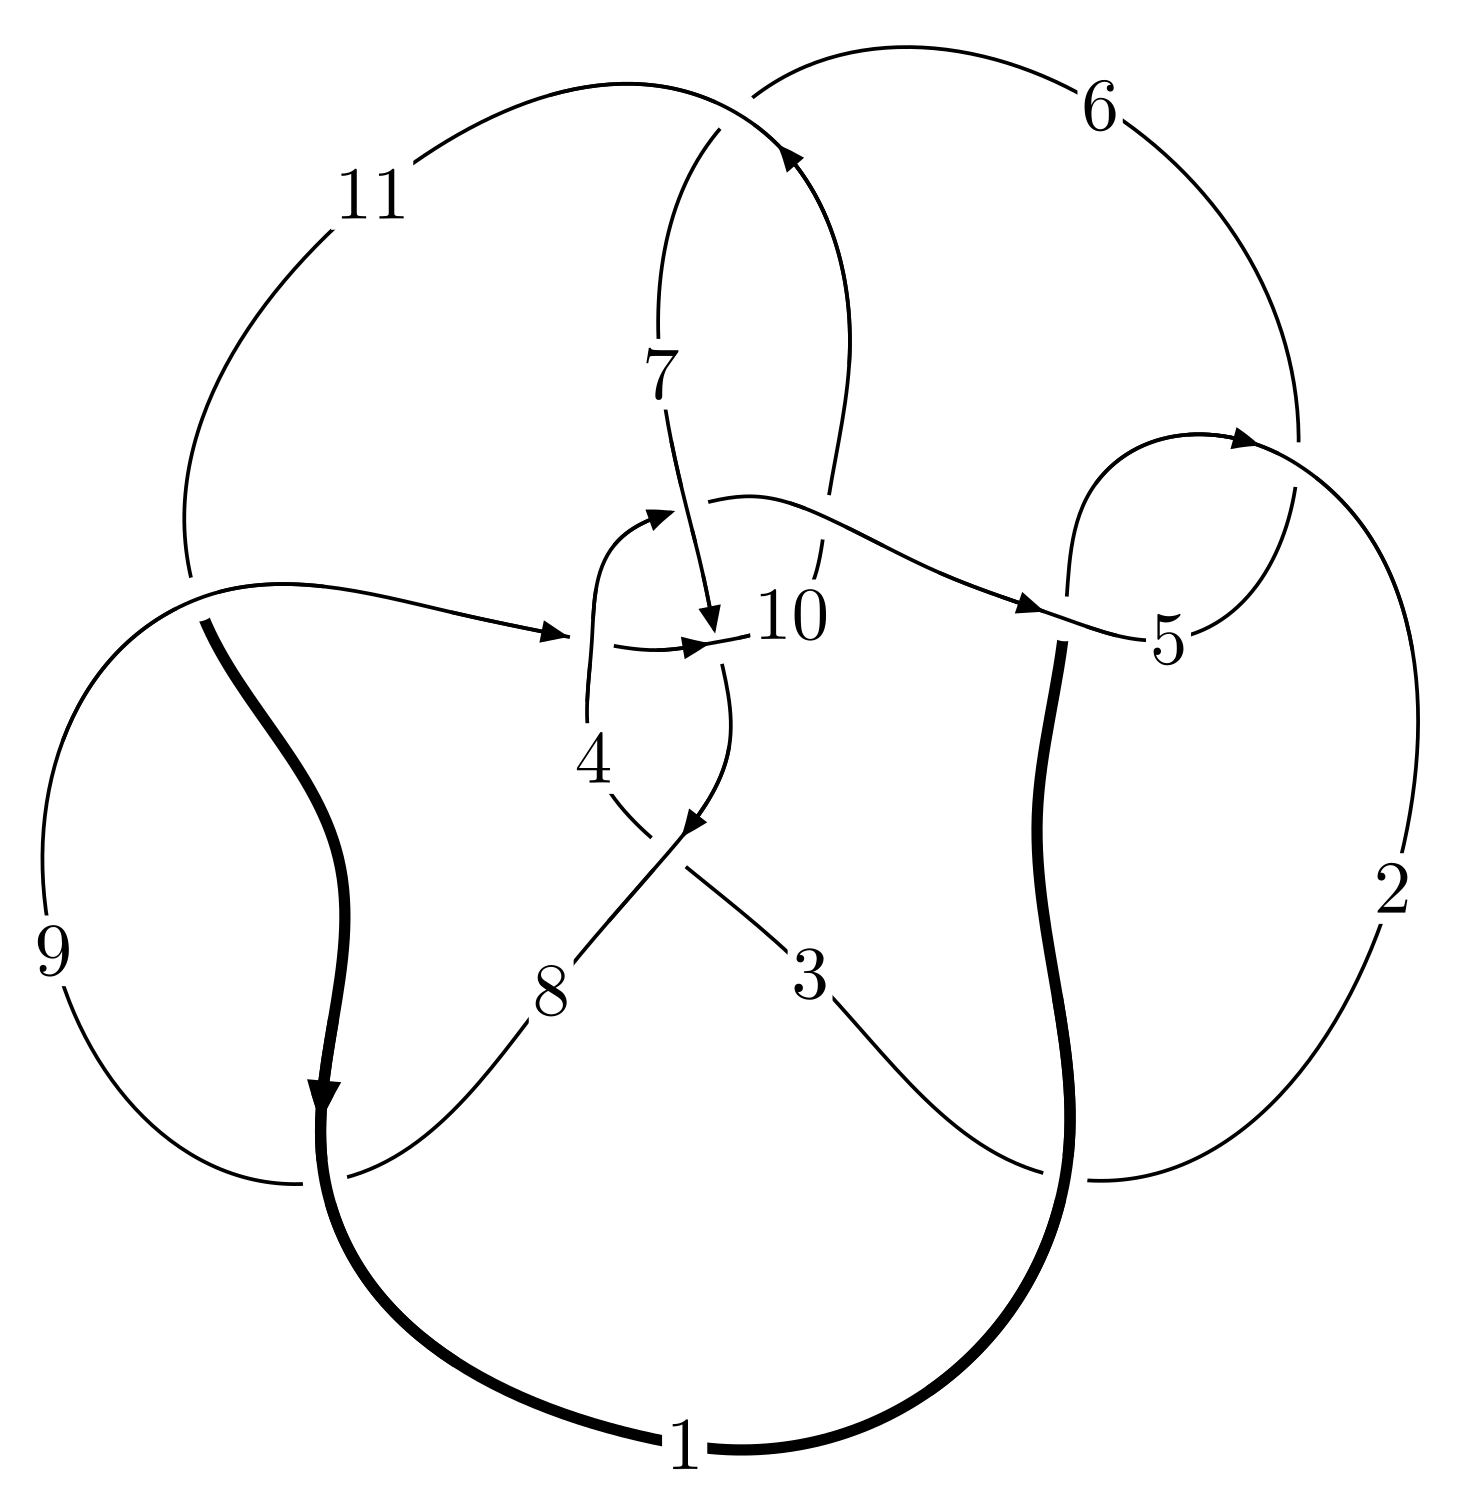
\includegraphics[width=112pt]{../../../GIT/diagram.site/Diagrams/png/712_11n_96.png}\\
\ \ \ A knot diagram\footnotemark}&
\allowdisplaybreaks
\textbf{Linearized knot diagam} \\
\cline{2-2}
 &
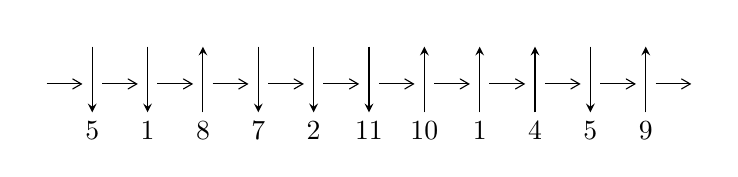
\begin{tikzpicture}[x=20pt, y=17pt]
	% nodes
	\node (C0) at (0, 0) {};
	\node (C1) at (1, 0) {};
	\node (C1U) at (1, +1) {};
	\node (C1D) at (1, -1) {5};

	\node (C2) at (2, 0) {};
	\node (C2U) at (2, +1) {};
	\node (C2D) at (2, -1) {1};

	\node (C3) at (3, 0) {};
	\node (C3U) at (3, +1) {};
	\node (C3D) at (3, -1) {8};

	\node (C4) at (4, 0) {};
	\node (C4U) at (4, +1) {};
	\node (C4D) at (4, -1) {7};

	\node (C5) at (5, 0) {};
	\node (C5U) at (5, +1) {};
	\node (C5D) at (5, -1) {2};

	\node (C6) at (6, 0) {};
	\node (C6U) at (6, +1) {};
	\node (C6D) at (6, -1) {11};

	\node (C7) at (7, 0) {};
	\node (C7U) at (7, +1) {};
	\node (C7D) at (7, -1) {10};

	\node (C8) at (8, 0) {};
	\node (C8U) at (8, +1) {};
	\node (C8D) at (8, -1) {1};

	\node (C9) at (9, 0) {};
	\node (C9U) at (9, +1) {};
	\node (C9D) at (9, -1) {4};

	\node (C10) at (10, 0) {};
	\node (C10U) at (10, +1) {};
	\node (C10D) at (10, -1) {5};

	\node (C11) at (11, 0) {};
	\node (C11U) at (11, +1) {};
	\node (C11D) at (11, -1) {9};
	\node (C12) at (12, 0) {};

	% arrows
	\draw[->,>={angle 60}]
	(C0) edge (C1) (C1) edge (C2) (C2) edge (C3) (C3) edge (C4) (C4) edge (C5) (C5) edge (C6) (C6) edge (C7) (C7) edge (C8) (C8) edge (C9) (C9) edge (C10) (C10) edge (C11) (C11) edge (C12) ;	\draw[->,>=stealth]
	(C1U) edge (C1D) (C2U) edge (C2D) (C3D) edge (C3U) (C4U) edge (C4D) (C5U) edge (C5D) (C6U) edge (C6D) (C7D) edge (C7U) (C8D) edge (C8U) (C9D) edge (C9U) (C10U) edge (C10D) (C11D) edge (C11U) ;
	\end{tikzpicture} \\
\hhline{~~} \\& 
\textbf{Solving Sequence} \\ \cline{2-2} 
 &
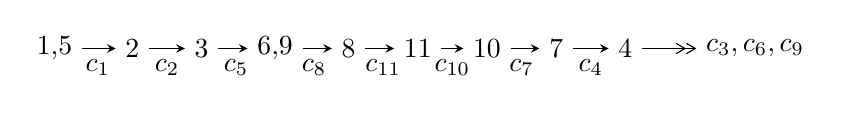
\begin{tikzpicture}[x=25pt, y=7pt]
	% node
	\node (A0) at (-1/8, 0) {1,5};
	\node (A1) at (1, 0) {2};
	\node (A2) at (2, 0) {3};
	\node (A3) at (49/16, 0) {6,9};
	\node (A4) at (33/8, 0) {8};
	\node (A5) at (41/8, 0) {11};
	\node (A6) at (49/8, 0) {10};
	\node (A7) at (57/8, 0) {7};
	\node (A8) at (65/8, 0) {4};
	\node (C1) at (1/2, -1) {$c_{1}$};
	\node (C2) at (3/2, -1) {$c_{2}$};
	\node (C3) at (5/2, -1) {$c_{5}$};
	\node (C4) at (29/8, -1) {$c_{8}$};
	\node (C5) at (37/8, -1) {$c_{11}$};
	\node (C6) at (45/8, -1) {$c_{10}$};
	\node (C7) at (53/8, -1) {$c_{7}$};
	\node (C8) at (61/8, -1) {$c_{4}$};
	\node (A9) at (10, 0) {$c_{3},c_{6},c_{9}$};

	% edge
	\draw[->,>=stealth]	
	(A0) edge (A1) (A1) edge (A2) (A2) edge (A3) (A3) edge (A4) (A4) edge (A5) (A5) edge (A6) (A6) edge (A7) (A7) edge (A8) ;
	\draw[->>,>={angle 60}]	
	(A8) edge (A9);
\end{tikzpicture} \\ 

\end{tabular} \\

\footnotetext{
The image of knot diagram is generated by the software ``\textbf{Draw programme}" developed by Andrew Bartholomew(\url{http://www.layer8.co.uk/maths/draw/index.htm\#Running-draw}), where we modified some parts for our purpose(\url{https://github.com/CATsTAILs/LinksPainter}).
}\phantom \\ \newline 
\centering \textbf{Ideals for irreducible components\footnotemark of $X_{\text{par}}$} 
 
\begin{align*}
I^u_{1}&=\langle 
-49163590906 u^{11}+107218013353 u^{10}+\cdots+21229569666128 b+7549955391253,\\
\phantom{I^u_{1}}&\phantom{= \langle  }-3432579931219 u^{11}+9265624647069 u^{10}+\cdots+891641925977376 a+779226085539559,\\
\phantom{I^u_{1}}&\phantom{= \langle  }u^{12}-18 u^{10}-3 u^9+95 u^8+104 u^7+172 u^6-39 u^5-97 u^4-126 u^3+90 u^2+56 u+21\rangle \\
I^u_{2}&=\langle 
u^4+2 u^3+b,\;2 u^4+4 u^3+u^2+a+3 u,\;u^5+3 u^4+3 u^3+3 u^2+2 u+1\rangle \\
I^u_{3}&=\langle 
-2 a^3- a^2+b-5 a+3,\;a^4+2 a^2-3 a+1,\;u-1\rangle \\
\\
\end{align*}
\raggedright * 3 irreducible components of $\dim_{\mathbb{C}}=0$, with total 21 representations.\\
\footnotetext{All coefficients of polynomials are rational numbers. But the coefficients are sometimes approximated in decimal forms when there is not enough margin.}
\newpage
\renewcommand{\arraystretch}{1}
\centering \section*{I. $I^u_{1}= \langle -4.92\times10^{10} u^{11}+1.07\times10^{11} u^{10}+\cdots+2.12\times10^{13} b+7.55\times10^{12},\;-3.43\times10^{12} u^{11}+9.27\times10^{12} u^{10}+\cdots+8.92\times10^{14} a+7.79\times10^{14},\;u^{12}-18 u^{10}+\cdots+56 u+21 \rangle$}
\flushleft \textbf{(i) Arc colorings}\\
\begin{tabular}{m{7pt} m{180pt} m{7pt} m{180pt} }
\flushright $a_{1}=$&$\begin{pmatrix}1\\0\end{pmatrix}$ \\
\flushright $a_{5}=$&$\begin{pmatrix}0\\u\end{pmatrix}$ \\
\flushright $a_{2}=$&$\begin{pmatrix}1\\u^2\end{pmatrix}$ \\
\flushright $a_{3}=$&$\begin{pmatrix}- u^2+1\\u^2\end{pmatrix}$ \\
\flushright $a_{6}=$&$\begin{pmatrix}- u\\- u^3+u\end{pmatrix}$ \\
\flushright $a_{9}=$&$\begin{pmatrix}0.00384973 u^{11}-0.0103916 u^{10}+\cdots+0.0171393 u-0.873923\\0.00231581 u^{11}-0.00505041 u^{10}+\cdots+0.944426 u-0.355634\end{pmatrix}$ \\
\flushright $a_{8}=$&$\begin{pmatrix}0.00153392 u^{11}-0.00534123 u^{10}+\cdots-0.927287 u-0.518289\\0.00231581 u^{11}-0.00505041 u^{10}+\cdots+0.944426 u-0.355634\end{pmatrix}$ \\
\flushright $a_{11}=$&$\begin{pmatrix}-0.00463890 u^{11}+0.00727890 u^{10}+\cdots-0.777940 u+1.33085\\-0.00697735 u^{11}+0.00595506 u^{10}+\cdots-0.776534 u+0.0957645\end{pmatrix}$ \\
\flushright $a_{10}=$&$\begin{pmatrix}-0.00463890 u^{11}+0.00727890 u^{10}+\cdots-0.777940 u+1.33085\\-0.00382620 u^{11}+0.00729647 u^{10}+\cdots-0.466333 u+0.248621\end{pmatrix}$ \\
\flushright $a_{7}=$&$\begin{pmatrix}-0.0229677 u^{11}+0.00971661 u^{10}+\cdots-4.00235 u-0.352817\\-0.00186562 u^{11}-0.00155113 u^{10}+\cdots+0.277243 u-0.308445\end{pmatrix}$ \\
\flushright $a_{4}=$&$\begin{pmatrix}-0.00384973 u^{11}+0.0103916 u^{10}+\cdots-0.0171393 u+0.873923\\0.00382620 u^{11}-0.00729647 u^{10}+\cdots+0.466333 u-0.248621\end{pmatrix}$\\ \flushright $a_{4}=$&$\begin{pmatrix}-0.00384973 u^{11}+0.0103916 u^{10}+\cdots-0.0171393 u+0.873923\\0.00382620 u^{11}-0.00729647 u^{10}+\cdots+0.466333 u-0.248621\end{pmatrix}$\\&\end{tabular}
\flushleft \textbf{(ii) Obstruction class $= -1$}\\~\\
\flushleft \textbf{(iii) Cusp Shapes $= \frac{6189983418965}{84918278664512} u^{11}+\frac{1650234375373}{84918278664512} u^{10}+\cdots+\frac{95722121856831}{84918278664512} u+\frac{414947504713599}{84918278664512}$}\\~\\
\newpage\renewcommand{\arraystretch}{1}
\flushleft \textbf{(iv) u-Polynomials at the component}\newline \\
\begin{tabular}{m{50pt}|m{274pt}}
Crossings & \hspace{64pt}u-Polynomials at each crossing \\
\hline $$\begin{aligned}c_{1},c_{5}\end{aligned}$$&$\begin{aligned}
&u^{12}-18 u^{10}+\cdots-56 u+21
\end{aligned}$\\
\hline $$\begin{aligned}c_{2}\end{aligned}$$&$\begin{aligned}
&u^{12}+36 u^{11}+\cdots-644 u+441
\end{aligned}$\\
\hline $$\begin{aligned}c_{3}\end{aligned}$$&$\begin{aligned}
&u^{12}+43 u^{10}+\cdots-242 u+713
\end{aligned}$\\
\hline $$\begin{aligned}c_{4}\end{aligned}$$&$\begin{aligned}
&u^{12}-3 u^{11}+4 u^{10}- u^9+u^8-6 u^7+8 u^6+u^5-5 u^4- u^3+4 u^2-3 u+1
\end{aligned}$\\
\hline $$\begin{aligned}c_{6}\end{aligned}$$&$\begin{aligned}
&u^{12}+2 u^{11}+\cdots+211 u+199
\end{aligned}$\\
\hline $$\begin{aligned}c_{7}\end{aligned}$$&$\begin{aligned}
&u^{12}+4 u^{11}+\cdots-56 u+48
\end{aligned}$\\
\hline $$\begin{aligned}c_{8},c_{11}\end{aligned}$$&$\begin{aligned}
&u^{12}+2 u^{11}+\cdots-2 u+1
\end{aligned}$\\
\hline $$\begin{aligned}c_{9}\end{aligned}$$&$\begin{aligned}
&u^{12}+9 u^{11}+\cdots+32 u+8
\end{aligned}$\\
\hline $$\begin{aligned}c_{10}\end{aligned}$$&$\begin{aligned}
&u^{12}- u^{11}+\cdots- u+1
\end{aligned}$\\
\hline
\end{tabular}\\~\\
\newpage\renewcommand{\arraystretch}{1}
\flushleft \textbf{(v) Riley Polynomials at the component}\newline \\
\begin{tabular}{m{50pt}|m{274pt}}
Crossings & \hspace{64pt}Riley Polynomials at each crossing \\
\hline $$\begin{aligned}c_{1},c_{5}\end{aligned}$$&$\begin{aligned}
&y^{12}-36 y^{11}+\cdots+644 y+441
\end{aligned}$\\
\hline $$\begin{aligned}c_{2}\end{aligned}$$&$\begin{aligned}
&y^{12}-268 y^{11}+\cdots+15582980 y+194481
\end{aligned}$\\
\hline $$\begin{aligned}c_{3}\end{aligned}$$&$\begin{aligned}
&y^{12}+86 y^{11}+\cdots-2050686 y+508369
\end{aligned}$\\
\hline $$\begin{aligned}c_{4}\end{aligned}$$&$\begin{aligned}
&y^{12}- y^{11}+\cdots- y+1
\end{aligned}$\\
\hline $$\begin{aligned}c_{6}\end{aligned}$$&$\begin{aligned}
&y^{12}-50 y^{11}+\cdots-181433 y+39601
\end{aligned}$\\
\hline $$\begin{aligned}c_{7}\end{aligned}$$&$\begin{aligned}
&y^{12}+14 y^{11}+\cdots+19136 y+2304
\end{aligned}$\\
\hline $$\begin{aligned}c_{8},c_{11}\end{aligned}$$&$\begin{aligned}
&y^{12}+30 y^{11}+\cdots-34 y+1
\end{aligned}$\\
\hline $$\begin{aligned}c_{9}\end{aligned}$$&$\begin{aligned}
&y^{12}-5 y^{11}+\cdots-160 y+64
\end{aligned}$\\
\hline $$\begin{aligned}c_{10}\end{aligned}$$&$\begin{aligned}
&y^{12}-31 y^{11}+\cdots+5 y+1
\end{aligned}$\\
\hline
\end{tabular}\\~\\
\newpage\flushleft \textbf{(vi) Complex Volumes and Cusp Shapes}
$$\begin{array}{c|c|c}  
\text{Solutions to }I^u_{1}& \I (\text{vol} + \sqrt{-1}CS) & \text{Cusp shape}\\
 \hline 
\begin{aligned}
u &= -0.695715 + 0.738682 I \\
a &= \phantom{-}0.84389 - 1.18718 I \\
b &= -0.353721 - 0.071932 I\end{aligned}
 & \phantom{-}0.40587 + 4.64089 I & \phantom{-}1.41872 - 4.81790 I \\ \hline\begin{aligned}
u &= -0.695715 - 0.738682 I \\
a &= \phantom{-}0.84389 + 1.18718 I \\
b &= -0.353721 + 0.071932 I\end{aligned}
 & \phantom{-}0.40587 - 4.64089 I & \phantom{-}1.41872 + 4.81790 I \\ \hline\begin{aligned}
u &= \phantom{-}0.778147 + 0.299444 I \\
a &= -0.811194 - 0.475700 I \\
b &= \phantom{-}0.333912 - 0.014682 I\end{aligned}
 & -1.39285 - 0.48352 I & -6.04456 + 0.14475 I \\ \hline\begin{aligned}
u &= \phantom{-}0.778147 - 0.299444 I \\
a &= -0.811194 + 0.475700 I \\
b &= \phantom{-}0.333912 + 0.014682 I\end{aligned}
 & -1.39285 + 0.48352 I & -6.04456 - 0.14475 I \\ \hline\begin{aligned}
u &= -0.182826 + 1.285270 I \\
a &= \phantom{-}0.012072 + 0.419952 I \\
b &= -0.18796 + 1.60199 I\end{aligned}
 & -4.09909 - 2.92553 I & -6.51732 + 0.13616 I \\ \hline\begin{aligned}
u &= -0.182826 - 1.285270 I \\
a &= \phantom{-}0.012072 - 0.419952 I \\
b &= -0.18796 - 1.60199 I\end{aligned}
 & -4.09909 + 2.92553 I & -6.51732 - 0.13616 I \\ \hline\begin{aligned}
u &= -0.246048 + 0.302553 I \\
a &= -0.835828 - 0.015119 I \\
b &= -0.578983 + 0.267705 I\end{aligned}
 & \phantom{-}1.34063 - 0.78648 I & \phantom{-}4.38906 + 1.25430 I \\ \hline\begin{aligned}
u &= -0.246048 - 0.302553 I \\
a &= -0.835828 + 0.015119 I \\
b &= -0.578983 - 0.267705 I\end{aligned}
 & \phantom{-}1.34063 + 0.78648 I & \phantom{-}4.38906 - 1.25430 I \\ \hline\begin{aligned}
u &= -3.01586 + 0.46060 I \\
a &= -0.161563 + 0.704724 I \\
b &= \phantom{-}0.81768 + 2.58567 I\end{aligned}
 & \phantom{-}18.0497 + 1.3274 I & -3.03771 + 0.06650 I \\ \hline\begin{aligned}
u &= -3.01586 - 0.46060 I \\
a &= -0.161563 - 0.704724 I \\
b &= \phantom{-}0.81768 - 2.58567 I\end{aligned}
 & \phantom{-}18.0497 - 1.3274 I & -3.03771 - 0.06650 I\\
 \hline 
 \end{array}$$\newpage$$\begin{array}{c|c|c}  
\text{Solutions to }I^u_{1}& \I (\text{vol} + \sqrt{-1}CS) & \text{Cusp shape}\\
 \hline 
\begin{aligned}
u &= \phantom{-}3.36230 + 0.99651 I \\
a &= -0.214046 - 0.589764 I \\
b &= \phantom{-}0.96907 - 2.80816 I\end{aligned}
 & \phantom{-}17.7719 - 9.0470 I & -3.20819 + 3.73893 I \\ \hline\begin{aligned}
u &= \phantom{-}3.36230 - 0.99651 I \\
a &= -0.214046 + 0.589764 I \\
b &= \phantom{-}0.96907 + 2.80816 I\end{aligned}
 & \phantom{-}17.7719 + 9.0470 I & -3.20819 - 3.73893 I\\
 \hline 
 \end{array}$$\newpage\newpage\renewcommand{\arraystretch}{1}
\centering \section*{II. $I^u_{2}= \langle u^4+2 u^3+b,\;2 u^4+4 u^3+u^2+a+3 u,\;u^5+3 u^4+3 u^3+3 u^2+2 u+1 \rangle$}
\flushleft \textbf{(i) Arc colorings}\\
\begin{tabular}{m{7pt} m{180pt} m{7pt} m{180pt} }
\flushright $a_{1}=$&$\begin{pmatrix}1\\0\end{pmatrix}$ \\
\flushright $a_{5}=$&$\begin{pmatrix}0\\u\end{pmatrix}$ \\
\flushright $a_{2}=$&$\begin{pmatrix}1\\u^2\end{pmatrix}$ \\
\flushright $a_{3}=$&$\begin{pmatrix}- u^2+1\\u^2\end{pmatrix}$ \\
\flushright $a_{6}=$&$\begin{pmatrix}- u\\- u^3+u\end{pmatrix}$ \\
\flushright $a_{9}=$&$\begin{pmatrix}-2 u^4-4 u^3- u^2-3 u\\- u^4-2 u^3\end{pmatrix}$ \\
\flushright $a_{8}=$&$\begin{pmatrix}- u^4-2 u^3- u^2-3 u\\- u^4-2 u^3\end{pmatrix}$ \\
\flushright $a_{11}=$&$\begin{pmatrix}- u^4-3 u^3-2 u^2- u-1\\u^4+3 u^3+3 u^2+2 u\end{pmatrix}$ \\
\flushright $a_{10}=$&$\begin{pmatrix}- u^4-3 u^3-2 u^2- u-1\\u^3+2 u^2+u\end{pmatrix}$ \\
\flushright $a_{7}=$&$\begin{pmatrix}u^3+2 u^2+u+2\\u^4+3 u^3+4 u^2+2 u\end{pmatrix}$ \\
\flushright $a_{4}=$&$\begin{pmatrix}2 u^4+4 u^3+u^2+3 u\\- u^3-2 u^2- u\end{pmatrix}$\\ \flushright $a_{4}=$&$\begin{pmatrix}2 u^4+4 u^3+u^2+3 u\\- u^3-2 u^2- u\end{pmatrix}$\\&\end{tabular}
\flushleft \textbf{(ii) Obstruction class $= 1$}\\~\\
\flushleft \textbf{(iii) Cusp Shapes $= -10 u^4-25 u^3-19 u^2-24 u-15$}\\~\\
\newpage\renewcommand{\arraystretch}{1}
\flushleft \textbf{(iv) u-Polynomials at the component}\newline \\
\begin{tabular}{m{50pt}|m{274pt}}
Crossings & \hspace{64pt}u-Polynomials at each crossing \\
\hline $$\begin{aligned}c_{1}\end{aligned}$$&$\begin{aligned}
&u^5+3 u^4+3 u^3+3 u^2+2 u+1
\end{aligned}$\\
\hline $$\begin{aligned}c_{2}\end{aligned}$$&$\begin{aligned}
&u^5+3 u^4-5 u^3+3 u^2-2 u+1
\end{aligned}$\\
\hline $$\begin{aligned}c_{3}\end{aligned}$$&$\begin{aligned}
&u^5- u^4-2 u^3+9 u^2-17 u+11
\end{aligned}$\\
\hline $$\begin{aligned}c_{4}\end{aligned}$$&$\begin{aligned}
&u^5-2 u^4+2 u^3+u^2-2 u+1
\end{aligned}$\\
\hline $$\begin{aligned}c_{5}\end{aligned}$$&$\begin{aligned}
&u^5-3 u^4+3 u^3-3 u^2+2 u-1
\end{aligned}$\\
\hline $$\begin{aligned}c_{6}\end{aligned}$$&$\begin{aligned}
&u^5+3 u^4-5 u^3-8 u^2+9 u+11
\end{aligned}$\\
\hline $$\begin{aligned}c_{7}\end{aligned}$$&$\begin{aligned}
&u^5+u^4-2 u^3+3 u^2+7 u+13
\end{aligned}$\\
\hline $$\begin{aligned}c_{8}\end{aligned}$$&$\begin{aligned}
&u^5- u^4+3 u^3-3 u^2+2 u-1
\end{aligned}$\\
\hline $$\begin{aligned}c_{9}\end{aligned}$$&$\begin{aligned}
&u^5- u^3+u^2+u-1
\end{aligned}$\\
\hline $$\begin{aligned}c_{10}\end{aligned}$$&$\begin{aligned}
&u^5+u^4- u^3- u^2+1
\end{aligned}$\\
\hline $$\begin{aligned}c_{11}\end{aligned}$$&$\begin{aligned}
&u^5+u^4+3 u^3+3 u^2+2 u+1
\end{aligned}$\\
\hline
\end{tabular}\\~\\
\newpage\renewcommand{\arraystretch}{1}
\flushleft \textbf{(v) Riley Polynomials at the component}\newline \\
\begin{tabular}{m{50pt}|m{274pt}}
Crossings & \hspace{64pt}Riley Polynomials at each crossing \\
\hline $$\begin{aligned}c_{1},c_{5}\end{aligned}$$&$\begin{aligned}
&y^5-3 y^4-5 y^3-3 y^2-2 y-1
\end{aligned}$\\
\hline $$\begin{aligned}c_{2}\end{aligned}$$&$\begin{aligned}
&y^5-19 y^4+3 y^3+5 y^2-2 y-1
\end{aligned}$\\
\hline $$\begin{aligned}c_{3}\end{aligned}$$&$\begin{aligned}
&y^5-5 y^4-12 y^3+9 y^2+91 y-121
\end{aligned}$\\
\hline $$\begin{aligned}c_{4}\end{aligned}$$&$\begin{aligned}
&y^5+4 y^3-5 y^2+2 y-1
\end{aligned}$\\
\hline $$\begin{aligned}c_{6}\end{aligned}$$&$\begin{aligned}
&y^5-19 y^4+91 y^3-220 y^2+257 y-121
\end{aligned}$\\
\hline $$\begin{aligned}c_{7}\end{aligned}$$&$\begin{aligned}
&y^5-5 y^4+12 y^3-63 y^2-29 y-169
\end{aligned}$\\
\hline $$\begin{aligned}c_{8},c_{11}\end{aligned}$$&$\begin{aligned}
&y^5+5 y^4+7 y^3+y^2-2 y-1
\end{aligned}$\\
\hline $$\begin{aligned}c_{9}\end{aligned}$$&$\begin{aligned}
&y^5-2 y^4+3 y^3-3 y^2+3 y-1
\end{aligned}$\\
\hline $$\begin{aligned}c_{10}\end{aligned}$$&$\begin{aligned}
&y^5-3 y^4+3 y^3-3 y^2+2 y-1
\end{aligned}$\\
\hline
\end{tabular}\\~\\
\newpage\flushleft \textbf{(vi) Complex Volumes and Cusp Shapes}
$$\begin{array}{c|c|c}  
\text{Solutions to }I^u_{2}& \I (\text{vol} + \sqrt{-1}CS) & \text{Cusp shape}\\
 \hline 
\begin{aligned}
u &= \phantom{-}0.128506 + 0.862169 I \\
a &= \phantom{-}0.520756 + 0.228796 I \\
b &= \phantom{-}0.08973 + 1.51845 I\end{aligned}
 & -3.58220 + 3.70382 I & -1.95503 - 6.72693 I \\ \hline\begin{aligned}
u &= \phantom{-}0.128506 - 0.862169 I \\
a &= \phantom{-}0.520756 - 0.228796 I \\
b &= \phantom{-}0.08973 - 1.51845 I\end{aligned}
 & -3.58220 - 3.70382 I & -1.95503 + 6.72693 I \\ \hline\begin{aligned}
u &= -0.586994 + 0.535944 I \\
a &= \phantom{-}1.27460 - 2.43458 I \\
b &= -0.214528 - 0.727972 I\end{aligned}
 & -0.27969 + 5.17259 I & -5.66442 - 10.18801 I \\ \hline\begin{aligned}
u &= -0.586994 - 0.535944 I \\
a &= \phantom{-}1.27460 + 2.43458 I \\
b &= -0.214528 + 0.727972 I\end{aligned}
 & -0.27969 - 5.17259 I & -5.66442 + 10.18801 I \\ \hline\begin{aligned}
u &= -2.08302\phantom{ +0.000000I} \\
a &= \phantom{-}0.409288\phantom{ +0.000000I} \\
b &= -0.750397\phantom{ +0.000000I}\end{aligned}
 & -5.43570\phantom{ +0.000000I} & -9.76110\phantom{ +0.000000I}\\
 \hline 
 \end{array}$$\newpage\newpage\renewcommand{\arraystretch}{1}
\centering \section*{III. $I^u_{3}= \langle -2 a^3- a^2+b-5 a+3,\;a^4+2 a^2-3 a+1,\;u-1 \rangle$}
\flushleft \textbf{(i) Arc colorings}\\
\begin{tabular}{m{7pt} m{180pt} m{7pt} m{180pt} }
\flushright $a_{1}=$&$\begin{pmatrix}1\\0\end{pmatrix}$ \\
\flushright $a_{5}=$&$\begin{pmatrix}0\\1\end{pmatrix}$ \\
\flushright $a_{2}=$&$\begin{pmatrix}1\\1\end{pmatrix}$ \\
\flushright $a_{3}=$&$\begin{pmatrix}0\\1\end{pmatrix}$ \\
\flushright $a_{6}=$&$\begin{pmatrix}-1\\0\end{pmatrix}$ \\
\flushright $a_{9}=$&$\begin{pmatrix}a\\2 a^3+a^2+5 a-3\end{pmatrix}$ \\
\flushright $a_{8}=$&$\begin{pmatrix}-2 a^3- a^2-4 a+3\\2 a^3+a^2+5 a-3\end{pmatrix}$ \\
\flushright $a_{11}=$&$\begin{pmatrix}a^3+a^2+3 a-1\\2 a^3+a^2+5 a-4\end{pmatrix}$ \\
\flushright $a_{10}=$&$\begin{pmatrix}a^3+a^2+3 a-1\\a^3+2 a-3\end{pmatrix}$ \\
\flushright $a_{7}=$&$\begin{pmatrix}-2 a^3- a^2-4 a+3\\2 a^3+a^2+5 a-3\end{pmatrix}$ \\
\flushright $a_{4}=$&$\begin{pmatrix}- a\\- a^3-2 a+3\end{pmatrix}$\\ \flushright $a_{4}=$&$\begin{pmatrix}- a\\- a^3-2 a+3\end{pmatrix}$\\&\end{tabular}
\flushleft \textbf{(ii) Obstruction class $= 1$}\\~\\
\flushleft \textbf{(iii) Cusp Shapes $= -5 a^3- a^2-11 a+6$}\\~\\
\newpage\renewcommand{\arraystretch}{1}
\flushleft \textbf{(iv) u-Polynomials at the component}\newline \\
\begin{tabular}{m{50pt}|m{274pt}}
Crossings & \hspace{64pt}u-Polynomials at each crossing \\
\hline $$\begin{aligned}c_{1}\end{aligned}$$&$\begin{aligned}
&(u-1)^4
\end{aligned}$\\
\hline $$\begin{aligned}c_{2},c_{5}\end{aligned}$$&$\begin{aligned}
&(u+1)^4
\end{aligned}$\\
\hline $$\begin{aligned}c_{3},c_{4}\end{aligned}$$&$\begin{aligned}
&u^4-2 u^3+2 u^2- u+1
\end{aligned}$\\
\hline $$\begin{aligned}c_{6},c_{11}\end{aligned}$$&$\begin{aligned}
&(u^2- u+1)^2
\end{aligned}$\\
\hline $$\begin{aligned}c_{7}\end{aligned}$$&$\begin{aligned}
&u^4
\end{aligned}$\\
\hline $$\begin{aligned}c_{8}\end{aligned}$$&$\begin{aligned}
&(u^2+u+1)^2
\end{aligned}$\\
\hline $$\begin{aligned}c_{9},c_{10}\end{aligned}$$&$\begin{aligned}
&u^4- u^3- u^2+u+1
\end{aligned}$\\
\hline
\end{tabular}\\~\\
\newpage\renewcommand{\arraystretch}{1}
\flushleft \textbf{(v) Riley Polynomials at the component}\newline \\
\begin{tabular}{m{50pt}|m{274pt}}
Crossings & \hspace{64pt}Riley Polynomials at each crossing \\
\hline $$\begin{aligned}c_{1},c_{2},c_{5}\end{aligned}$$&$\begin{aligned}
&(y-1)^4
\end{aligned}$\\
\hline $$\begin{aligned}c_{3},c_{4}\end{aligned}$$&$\begin{aligned}
&y^4+2 y^2+3 y+1
\end{aligned}$\\
\hline $$\begin{aligned}c_{6},c_{8},c_{11}\end{aligned}$$&$\begin{aligned}
&(y^2+y+1)^2
\end{aligned}$\\
\hline $$\begin{aligned}c_{7}\end{aligned}$$&$\begin{aligned}
&y^4
\end{aligned}$\\
\hline $$\begin{aligned}c_{9},c_{10}\end{aligned}$$&$\begin{aligned}
&y^4-3 y^3+5 y^2-3 y+1
\end{aligned}$\\
\hline
\end{tabular}\\~\\
\newpage\flushleft \textbf{(vi) Complex Volumes and Cusp Shapes}
$$\begin{array}{c|c|c}  
\text{Solutions to }I^u_{3}& \I (\text{vol} + \sqrt{-1}CS) & \text{Cusp shape}\\
 \hline 
\begin{aligned}
u &= \phantom{-}1.00000\phantom{ +0.000000I} \\
a &= \phantom{-}0.570696 + 0.107280 I \\
b &= \phantom{-}0.500000 + 0.866025 I\end{aligned}
 & -1.64493 + 2.02988 I & -1.42268 - 1.82047 I \\ \hline\begin{aligned}
u &= \phantom{-}1.00000\phantom{ +0.000000I} \\
a &= \phantom{-}0.570696 - 0.107280 I \\
b &= \phantom{-}0.500000 - 0.866025 I\end{aligned}
 & -1.64493 - 2.02988 I & -1.42268 + 1.82047 I \\ \hline\begin{aligned}
u &= \phantom{-}1.00000\phantom{ +0.000000I} \\
a &= -0.57070 + 1.62477 I \\
b &= \phantom{-}0.500000 + 0.866025 I\end{aligned}
 & -1.64493 + 2.02988 I & -7.07732 - 2.50966 I \\ \hline\begin{aligned}
u &= \phantom{-}1.00000\phantom{ +0.000000I} \\
a &= -0.57070 - 1.62477 I \\
b &= \phantom{-}0.500000 - 0.866025 I\end{aligned}
 & -1.64493 - 2.02988 I & -7.07732 + 2.50966 I\\
 \hline 
 \end{array}$$\newpage
\newpage\renewcommand{\arraystretch}{1}
\centering \section*{ IV. u-Polynomials}
\begin{tabular}{m{50pt}|m{274pt}}
Crossings & \hspace{64pt}u-Polynomials at each crossing \\
\hline $$\begin{aligned}c_{1}\end{aligned}$$&$\begin{aligned}
&((u-1)^4)(u^5+3 u^4+\cdots+2 u+1)(u^{12}-18 u^{10}+\cdots-56 u+21)
\end{aligned}$\\
\hline $$\begin{aligned}c_{2}\end{aligned}$$&$\begin{aligned}
&(u+1)^4(u^5+3 u^4-5 u^3+3 u^2-2 u+1)\\
&\cdot(u^{12}+36 u^{11}+\cdots-644 u+441)
\end{aligned}$\\
\hline $$\begin{aligned}c_{3}\end{aligned}$$&$\begin{aligned}
&(u^4-2 u^3+2 u^2- u+1)(u^5- u^4-2 u^3+9 u^2-17 u+11)\\
&\cdot(u^{12}+43 u^{10}+\cdots-242 u+713)
\end{aligned}$\\
\hline $$\begin{aligned}c_{4}\end{aligned}$$&$\begin{aligned}
&(u^4-2 u^3+2 u^2- u+1)(u^5-2 u^4+2 u^3+u^2-2 u+1)\\
&\cdot(u^{12}-3 u^{11}+4 u^{10}- u^9+u^8-6 u^7+8 u^6+u^5-5 u^4- u^3+4 u^2-3 u+1)
\end{aligned}$\\
\hline $$\begin{aligned}c_{5}\end{aligned}$$&$\begin{aligned}
&((u+1)^4)(u^5-3 u^4+\cdots+2 u-1)(u^{12}-18 u^{10}+\cdots-56 u+21)
\end{aligned}$\\
\hline $$\begin{aligned}c_{6}\end{aligned}$$&$\begin{aligned}
&(u^2- u+1)^2(u^5+3 u^4-5 u^3-8 u^2+9 u+11)\\
&\cdot(u^{12}+2 u^{11}+\cdots+211 u+199)
\end{aligned}$\\
\hline $$\begin{aligned}c_{7}\end{aligned}$$&$\begin{aligned}
&u^4(u^5+u^4+\cdots+7 u+13)(u^{12}+4 u^{11}+\cdots-56 u+48)
\end{aligned}$\\
\hline $$\begin{aligned}c_{8}\end{aligned}$$&$\begin{aligned}
&((u^2+u+1)^2)(u^5- u^4+\cdots+2 u-1)(u^{12}+2 u^{11}+\cdots-2 u+1)
\end{aligned}$\\
\hline $$\begin{aligned}c_{9}\end{aligned}$$&$\begin{aligned}
&(u^4- u^3- u^2+u+1)(u^5- u^3+u^2+u-1)(u^{12}+9 u^{11}+\cdots+32 u+8)
\end{aligned}$\\
\hline $$\begin{aligned}c_{10}\end{aligned}$$&$\begin{aligned}
&(u^4- u^3- u^2+u+1)(u^5+u^4- u^3- u^2+1)(u^{12}- u^{11}+\cdots- u+1)
\end{aligned}$\\
\hline $$\begin{aligned}c_{11}\end{aligned}$$&$\begin{aligned}
&((u^2- u+1)^2)(u^5+u^4+\cdots+2 u+1)(u^{12}+2 u^{11}+\cdots-2 u+1)
\end{aligned}$\\
\hline
\end{tabular}\newpage\renewcommand{\arraystretch}{1}
\centering \section*{ V. Riley Polynomials}
\begin{tabular}{m{50pt}|m{274pt}}
Crossings & \hspace{64pt}Riley Polynomials at each crossing \\
\hline $$\begin{aligned}c_{1},c_{5}\end{aligned}$$&$\begin{aligned}
&(y-1)^4(y^5-3 y^4-5 y^3-3 y^2-2 y-1)\\
&\cdot(y^{12}-36 y^{11}+\cdots+644 y+441)
\end{aligned}$\\
\hline $$\begin{aligned}c_{2}\end{aligned}$$&$\begin{aligned}
&(y-1)^4(y^5-19 y^4+3 y^3+5 y^2-2 y-1)\\
&\cdot(y^{12}-268 y^{11}+\cdots+15582980 y+194481)
\end{aligned}$\\
\hline $$\begin{aligned}c_{3}\end{aligned}$$&$\begin{aligned}
&(y^4+2 y^2+3 y+1)(y^5-5 y^4-12 y^3+9 y^2+91 y-121)\\
&\cdot(y^{12}+86 y^{11}+\cdots-2050686 y+508369)
\end{aligned}$\\
\hline $$\begin{aligned}c_{4}\end{aligned}$$&$\begin{aligned}
&(y^4+2 y^2+3 y+1)(y^5+4 y^3+\cdots+2 y-1)(y^{12}- y^{11}+\cdots- y+1)
\end{aligned}$\\
\hline $$\begin{aligned}c_{6}\end{aligned}$$&$\begin{aligned}
&(y^2+y+1)^2(y^5-19 y^4+91 y^3-220 y^2+257 y-121)\\
&\cdot(y^{12}-50 y^{11}+\cdots-181433 y+39601)
\end{aligned}$\\
\hline $$\begin{aligned}c_{7}\end{aligned}$$&$\begin{aligned}
&y^4(y^5-5 y^4+12 y^3-63 y^2-29 y-169)\\
&\cdot(y^{12}+14 y^{11}+\cdots+19136 y+2304)
\end{aligned}$\\
\hline $$\begin{aligned}c_{8},c_{11}\end{aligned}$$&$\begin{aligned}
&(y^2+y+1)^2(y^5+5 y^4+7 y^3+y^2-2 y-1)\\
&\cdot(y^{12}+30 y^{11}+\cdots-34 y+1)
\end{aligned}$\\
\hline $$\begin{aligned}c_{9}\end{aligned}$$&$\begin{aligned}
&(y^4-3 y^3+5 y^2-3 y+1)(y^5-2 y^4+3 y^3-3 y^2+3 y-1)\\
&\cdot(y^{12}-5 y^{11}+\cdots-160 y+64)
\end{aligned}$\\
\hline $$\begin{aligned}c_{10}\end{aligned}$$&$\begin{aligned}
&(y^4-3 y^3+5 y^2-3 y+1)(y^5-3 y^4+3 y^3-3 y^2+2 y-1)\\
&\cdot(y^{12}-31 y^{11}+\cdots+5 y+1)
\end{aligned}$\\
\hline
\end{tabular}
\vskip 2pc
\end{document}